
\documentclass[12pt,oneside,a4paper,leqno]{article}
\usepackage{appendix}
\usepackage{amsmath}
\usepackage{caption}
\usepackage{placeins}
\usepackage{graphicx}
\usepackage{subcaption}
%\usepackage{pgf}
\usepackage{tikz}

%\setlength\PreviewBorder{5pt}
\usepackage{natbib}
\bibpunct{(}{)}{,}{a}{}{;} 
\usepackage{url}
\usepackage{nth}
% for the d in integrals
\newcommand{\dd}{\; \mathrm{d}}
\newcommand{\ec}{\quad\quad\text{,}}
\newcommand{\ep}{\quad\quad\text{.}}
\defcitealias{HMD}{HMD}
\usepackage[top=2in, bottom=1.5in, left=1in, right=1in]{geometry}
\usepackage{setspace}
\doublespacing

\newcommand\ackn[1]{%
  \begingroup
  \renewcommand\thefootnote{}\footnote{#1}%
  \addtocounter{footnote}{-1}%
  \endgroup
}

% matrix numbering
\usepackage{trivfloat}
\trivfloat{matrix}
\floatstyle{plaintop}
    \restylefloat{matrix}
\AtBeginDocument{\numberwithin{matrix}{section}}

\newcommand{\Py}[2]{\includegraphics[scale=.5]{Figures/MiniPyramids/{Pyr-r#1-e0#2}.pdf}}
\newcommand{\Lf}[2]{\includegraphics[scale=.5]{Figures/MiniPyramids/{Leaf-r#1-e0#2}.pdf}}
% end preamble
%-------------------------------------------------------
\begin{document}

\title{Renewal and stability in populations structured by remaining years of
life}
\author{(author redacted)}
\maketitle


%\ackn{Research
%reported in this manuscript was supported by the U.S.
%National Institute On Aging of the National Institutes of Health under award
% numbers R01-AG011552 and R01-AG040245. The content is solely the responsibility of the author and does not necessarily represent the official views of the funding
%agency.}


\section*{Structured abstract}

\subsection*{Background}
The Lotka-Leslie renewal model is the core of formal demography. This model is
structured by age, and it does not account for time until death.

\subsection*{Objective}
I derive a specification of the classic renewal equation that is structured by
years left rather than by years lived. I give both continuous
and discrete variants of the derived model, and relate these to the Lotka-Leslie
renewal model.

\subsection*{Results}
In stability, the years lived and left renewal models are
commensurable, implying identical intrinsic growth rates.
I demonstrate approximate symmetry between years lived and left age structure in
stability when subject to intrinsic growth rates of equal magnitude and opposite
sign.

\subsection*{Conclusions}
Birth-death renewal processes can be expressed as death-birth processes, and
vice versa.

\subsection*{Contribution}
The years-left renewal model offers a new perspective on population renewal.
\vspace{2cm}

\section*{Introduction}
Contemporary demography is built upon a small set of empirically regular age
patterns. The models and methods
of demography are in varying degrees prefaced on such regularity. There is evidence that many demographic phenomena are best described in the
aggregatate as a function of time since birth, and others of time until death,
while others can be a function of both to some degree
\citep{riffe2015ttd,wolf2015disability}. Further, aggregate indices
motivated by measures of remaining lifetime have also become widely-used
indicators of ageing \citep{sanderson2007new}. These observations motivate
incorporating time-to-death into formal demographic methods and models.

In this paper, I explore some formal demographic consequences of a particular
redefinition of age. Instead of counting age as the time passed since birth,
consider the amount of time left until death.\footnote{Elsewhere this quantity
is referred to as \textit{residual} life, time-to-death (TTD), prospective
age \citep{sanderson2007new}, or thanatological age \citep{riffe2015force}.}
Individuals in this case move in the same direction along imaginary life lines,
but the reference point for measurement is switched from birth to death. For
individuals, the timing of events in life is exactly identified using either of
years lived or left, but aggregate patterns differ.
%Temporal perspectives and rescalings of the lifecourse are abundant in
% demography already. Such work has enriched the discipline by producing new
% insights, questions, and conundrums.
% Fertility and reproduction are plausibly a function of both age perspectives,
 % and the question of how to best partition them over time is not investigated here. 

The renewal model relates
fertility, mortality, and population structure in a parsimonious form, revealing
the long term consequences of a set of vital rates. All lines
of contemporary demographic research are relatable to the renewal model, and by
extention to stable population theory. The purpose of this paper is to describe
the Lotka-Leslie renewal model when structured by years of life left.
%Some might say that stable population
%theory is not relevant to everyday demography, since populations are always
% changing. Even if change precludes the notion of stability as a prediction, models of long-run consequnces still give a
%useful measure of the demographic force implied by a given set of rates.
%In this and other ways, stability is never far away. That population
% projections lead into a stable state means that some form of stability is implied by the routine practice of demography.
%Stability or even stationarity are imaginable for the world population of
% humans one day. Models of stationary populations are easily applied by analogy to
%closed or nearly-closed birth cohorts. Finally, stable population theory is
%relavant for modelling some non-human populations. 
%We have stated that many lifecourse transitions covary more with remaining
%lifetime than with life lived. In an even more general sense, by thinking about
% remaining lifetime as a particular class of time-to-transition, one may generalize the lifetable methods presented here into new area applications, such as education, partnering, the economic lifecycle, or migration.
%To present the renewal model based on thanatological age is not necessarily a
%suggestion for a better way to model or project population. Rather, 
The years-left renewal model represents an alternative and coherent way to
describe the process of population renewal by relating renewal to a death flow
rather than to a birth flow. I have described a limited case of this
perspective on renewal for the case of stationary populations
\citep{riffe2015force}, and here provide a broader treatment allowing for
growth in the population.
The years-lived renewal model and the years-left renewal
model both describe the movement of population stocks over time, but from opposite vantage points. %Specifying a model of thanatological renewal expands the toolbox available to approach complex temporal population structure. 

I couch the present inquiry in terms of aggregate renewal of human populations,
but the renewal model is more generally a description of the birth-death
process \citep{cox1962,feller1941integral}, and so may be valid for other kinds
of renewable aggregates.
The present inquiry establishes the validity of the model, but does not argue
for its empirical practicality or soundness.
%Perhaps there exists a birth-death process for which modelling as a death-birth
% process makes the most sense. In order to establish the \textit{soundness} of this model as a description of the human renewal process
%would require considerable empirical groundwork--- It would imply demonstrating
%that the thanatological age pattern of fertility is empirically regular, and
%that the time-to-death structure of the population is empirically regular.
%Such an endeavor would be misplaced, as the objective of this inquiry is not to
%improve the practice of empirical demography. 
The years lived and left renewal models imply one another in the state of stability. We
therefore present the years left model as a property implied by the
standard Lotka-Leslie renewal model, as two sides of the same coin. The objective in this paper is to deepen
our understanding of the Lotka-Leslie renewal model, and to offer an extention
of stable population theory.

The next section of this article reviews the lifetable method of transforming
age-classified data into remaining years classes. I then derive the continuous version of
the years left renewal model, and some other stable properties. This is
followed by the matrix version of the model, which is explained alongside the
lifecycle graph. Finally, I explore patterns in stable age structure compared
between the two models. I conclude that years left renewal offers
a new perspective on the familiar Lotka-Leslie model.

\section*{Requisites of a years-left renewal model}
The Lotka-Leslie renewal model \citep{sharpe1911problem, leslie1945use} is
situated in a closed, unisex, homogenous population framework. With
parameters equated, the continuous form of the model contains a component for
survival, $\ell(a)$, a scaling factor for growth, $e^{-ra}$, and a component for fertility, $m(a)$:

\begin{equation}
\label{eq:lotka}
1 = \int_{a=0}^\infty l(a)e^{-ra}m(a)\dd a \ep
\end{equation}

Each of these elements is structured by
age, $a$. The model can be approximated by observed data because
age is typically known. % The survival function, $\ell(a)$, derives
%from a lifetable, usually based on age-specific event-exposure mortality rates,
%which require counts of decedents and an estimate of the
%population exposed to risk in the same chronological age classes.
Age in the growth factor, $e^{-ra}$, pertains to the passage of
time more than it does to chronological age (this is synchronous with birth
cohorts). The product of this growth factor and $\ell(a)$ gives a
function proportional to the stable age structure, $c(a)$, and it is often
intuitive to imagine these two elements together as one for this reason. Female
fertility rates, $m(a)$, are based on daughters born to mothers in this limited
single-sex model. The functions $m(a)$ and $\ell(a)$
together intuitively make for net female fertility, and their age-wise product
is sometimes written as $\phi(a)$. This model lends itself to commonly collected data because age
is typically known, and can be asked.
% For the two essential rate componenents underlying the renewal
 % equation~\eqref{eq:lotka}, classification by chronological age is essentially given--- it is deterministic in the sense that time passed since birth is typically known by individuals. The kinds of errors in such classification are mostly due to innumeracy, rounding, exaggeration, and similar kinds of biases, but even in such cases, chronological age is fundamentally knowable.

Remaining lifetime is different in this respect because we do not know when we
will die--- it is only knowable retrospectively or probabilistically. Under a set of simple assumptions, the same lifetable used to
estimate $\ell(a)$ can be used to
partition and recombine counts observed by age into estimates
classified by years of life left. Our objective is then to estimate a population
structure component, similar to $\ell(a)e^{-ra}$, and a fertility component
similar to $m(a)$, but each for the years left case. Taken together, these
componenents yield the years left renewal model.

\subsection*{A lifetable approximation of life left}
%Direct information on the timing of demographic transitions with respect to
%death is available retrospectively from linked population registers or
%panel surveys with mortality follow-ups.
%Some surveys also ask respondents in various ways about their perceived future
% lifetime, which may underly those demographic transitions governed to some degree by volition. 

%In general, to make a lifetable-based projective statement about the remaining
%time distribution of a current stock of population, it is best to to account
% for population subgroups with different mortality and to account for uncertainty about future changes in
%mortality.
The present inquiry approximates years left in the aggregate using
lifetable-projected remaining lifetime, which is intended to approximate remaining lifetime under the strong
assumptions of homogenous populations und fixed vital rates. 
%Chronological age-classified counts are redistributed over future death times
% according to a fixed mortality schedule.
%In general, a lifetable approach to transforming chronologically classified
%data into thanatologically classified data is sound if the given lifetable
%accurately describes the future mortality of the age-classified population, and
%if the chronological and thantological age patterns are independent.
Under these assumptions, each birth cohort undergoes the same
pattern of attrition. %In a period setting, this means that we can distribute
% the remaining lifespans of the population in each age class using the same
%lifetable.
%This is the case we explore, and so the following formulas assume a single lifetable pattern.

The basic transformation to years left starts with the well-known remaining
years density function, $f(y|a)$.
%For age zero, $f(y|0)$ is identical to $d(a)$, the lifetable deaths
% distribution (based on a unity radix).
%For ages higher than 0, simply condition on survival:
%\footnote{In the
% reliability literature, $f(y|a)$ is denoted by $ X - t | X > t $, where $X$ is the total lifespan and $t$ is the
%current chronological age attained.}
\begin{equation}
\label{eq:vaupel1}
f(y | a) = \mu(a+y)\frac{\ell(a+y)}{\ell(a)} \ec
\end{equation}
where $\mu(a)$ is the force of mortality.
%A convenient discretization of \eqref{eq:vaupel1} is to simply work with the
%$d_a$ column of the lifetable (here with single ages):
%\begin{equation}
%\label{eq:dyadiscret}
%f_{y, a} =  \frac{d_{a+y}+d_{a+y+1}}{L_a + L_{a+1}} \ec
%\end{equation}
%where $L_a$ is lifetable exposure.\footnote{Equation~\eqref{eq:dyadiscret}
%will incur some error depending on the method used to derive $L_a$. To remove
%this error, rescale over the $a$ margin so that each distribution conditioned
% on $a$ sums to 1. Working with $\ell_a$ rather than $L_a$ eliminates error and
%yields similar results, but is not necessarily better.} One produces in this
% way a probability density function over future death times for each chronological age, $a$. 
The $f(y|a)$- weighted average of $y$ for a given $a$ returns the remaining life
expectancy column of the lifetable, $e(a)$. $f(y|a)$ is also useful for
decomposing age-classified data, such as the
population pyramid, into remaining years classes. If $P(a)$ is an
age-classified population count, we can derive the years left version $P(y)$,
using\footnote{An identical definition is found in
\citet{brouard1989mouvements} and illustrated in \citet{brouard1986structure}.}

\begin{align}
\label{eq:transform}
P(y) =& \int_0^\infty P(a) f(y | a) \dd a \ep
\end{align}

Figure~\ref{fig:pop} shows this exercise for 2010 US data \citep{HMD},
assuming homogeneity and that the 2010 period mortality schedule is held fixed.
When looking from the age perspective (Figure~\ref{fig:USdecomp}), this
decomposition reveals projected years left heterogeneity within a stock of known age, but when viewed from the
years left perspective (Figure~\ref{fig:USrecomp}) it reveals age heterogeneity
and the projected overall years left profile--- the future death flow of the
current population, $P(y)$ under our assumptions.

% both figures created in R/Pyramids.R
\begin{figure}[ht!]
	\caption{2010 US population structure}
	\label{fig:pop}
	\begin{center}
	\begin{subfigure}{.45\textwidth}
		\caption{Age structure (years lived) decomposed by years left.}
		\label{fig:USdecomp}
		\includegraphics[scale=.6]{Figures/US2010Age.pdf}
	\end{subfigure}
	~
	\begin{subfigure}{.45\textwidth}
		\caption{Years left structure decomposed by years lived.}
		\label{fig:USrecomp}
		\includegraphics[scale=.6]{Figures/US2010Thano.pdf}
	\end{subfigure}
	\\
	\small{*Population and mortality data from the HMD.}
	\end{center}
\end{figure}

\citet{brouard1986structure} applied this method to highlight regional
differences in French age structure, at times combining this projective method
with historical stocks. \citet{brouard1989mouvements}, and \citet{vaupel2009life}, showed that in stationary populations the
marginal chronological and thanatological age structures are identical, and this
provides a limited basis for comparison between the two perspectives. 
%\citet{wachter2014essential} hints at, and
%\citet{vaupel2014stable} elaborates on how to make chronological and
%thanatological age structure commensurate under a constant growth rate, $r$.
%These results also follow from the following specification of a
%thanatological renewal model.

Lifetable-derived thanatological age structure is
probabilistic until after death in several senses. In this case, note that
counts from a given age class are distributed over a range of higher ages
according to a given mortality rate schedule; in this
case a period mortality pattern is used.
As such, Figure~\ref{fig:USrecomp} is \textit{projective} in nature, a
forward-looking glance at population attrition given the population stock and lifetable of a
particular moment, whereas Figure~\ref{fig:USdecomp} is \textit{reflective} in
nature, since a population's chronological age-structure is the fruit of past
demographic forces.

\subsection{Thanatological fertility rates.}
Any count
classified by chronological age can be reclassified as in
equation~\eqref{eq:transform} given a pertinent lifetable. To
derive thanatological fertility rates under these assumptions, $\gamma(y)$, apply \eqref{eq:transform} to
chronological age-classified birth counts, $B(a)$, to get $B(y)$ and again to
exposure-to-risk, $E(a)$, to get $E(y)$ and then divide in the usual way:

\begin{equation}
\gamma(y) = \frac{B(y}{E(y)} \ep
\end{equation}

Figure~\ref{fig:FySpaghetti}
represents the full variety in female thanatological period fertility rates that can be found for all years
of data that overlap in the HFD and HMD.\footnote{There are as of this writing
1933 population-years of overlap between the HMD and HFD, including a wide
variety of fertility and mortality combinations.} I show $\gamma(y)$ calculated in this way because
it enters into the renewal model here studied. Figure~\ref{fig:FxSpaghetti}
gives ASFR for the same populations and years as a more familiar reference, but
note that both the x and y axes are different. The shape of thanatological
fertility curves is speculative and due to the above-mentioned strong assumptions. Nonetheless it is best not to
include such rates into a model blindly, so we offer this schematic overview of
some of their characteristics.

Period thanatological fertility rates estimated in this way have a
characteristic shape. The distribution is wider than that of chronological
fertility rates. The range of post-childbearing lifespans stretches from 
zero, due e.g., to maternal mortality, to at least 100.\footnote{For instance,
Jeanne Calment lived for another 100 years after giving birth to her daughter.}
This spaghetti plot includes both fertility booms and busts, as well as some
mortality crises (1918, WWII). Some patterns in the data (not
highlighted in the figure) include that the left tail (a gauge of how
orphan-prone a population is) has tended to fall over time. All populations have shown an increase in both the
mean and mode of thanatological age at childbearing over time. Several
contemporary populations now show modes of over 60 years. Period thanatological total
fertility rates track standard period total fertility rates closely, but tend to be somewhat higher (not shown).
% both figures created in R/HFDspaghetti.R
\begin{figure}[h!]
	\caption{Chronological and thantological fertility rates, all 1933
	country-year combinations present in both the HFD and HMD.* Note different x
	and y scales.}
	\label{fig:Fxcompare}
	\begin{center}
	\makebox[\textwidth]{
	\begin{subfigure}{.45\textwidth}
		\caption{Chronological period fertility rates.}
		\label{fig:FxSpaghetti}
		\includegraphics[scale=.45]{Figures/FxSpaghettiDraft.png}
	\end{subfigure}
	~
	\begin{subfigure}{.45\textwidth}
		\caption{Thanatological period fertility rates.}
		\label{fig:FySpaghetti}
		\includegraphics[scale=.45]{Figures/FySpaghettiDraft.png}
	\end{subfigure}
	}
	\\
	\end{center}
	\begin{tiny}
	*AUT, $1951-2010$; BGR, $1947-2009$; BLR, $1964-2012$; CAN, $1921-2009$; 
	CHE, $1932-2011$; CHL, $1992-2005$; CZE, $1950-2011$; DEUTE, $1956-2011$; 
	DEUTNP, $1990-2011$; DEUTW, $1956-2011$; ESP, $1922-2012$; EST, $1959-2011$; 
	FIN, $1939-2009$; FRATNP, $1946-2013$; GBR\_NIR, $1974-2011$; GBR\_NP,
	$1974-2011$; GBR\_SCO, $1945-2011$; GBRTENW, $1938-2011$; HUN, $1950-2009$;
	IRL, $1955-2009$; ISL, $1963-2010$; JPN, $1947-2012$; LTU, $1959-2011$; NLD, $1950-2009$; 
	NOR, $1967-2009$; PRT, $1940-2012$; RUS, $1959-2010$; SVK, $1950-2009$; 
	SVN, $1983-2009$; SWE, $1891-2011$; TWN, $1976-2010$; UKR, $1959-2009$; 
	USA, $1933-2010$
	\end{tiny}
\end{figure}

In general, thanatological fertility rates will not be useful for purposes of
projection, unless their empirical regularity is
stronger than typical ASFR. This is a question I do not seek to answer
in the present treatment, but in any case such rates are not susceptible to
direct measurement.
There are alternative ways of defining thanatological fertility rates, for instance by transforming the birth and
population vector from a stable population. As proven in appendix~\ref{app:B},
thanatological fertility rates derived from a stable population imply a certain
symmetry with stable populations from the chronological model. 

\FloatBarrier
\section*{The thanatological renewal model}
The renewal model that follows uses thanatological fertility rates, $\gamma(y)$,
the form of which is suggested in Figure~\ref{fig:FySpaghetti}, and we refer to
a homogenous, closed, unisex population based on female vital rates. Assuming constant vital rates, the births for the present year are given by 
\begin{align}
B(t) =& \int _0^\infty P(y,t)\gamma(y) \dd y = \int _0^\infty
P(a,t)m(a) \dd a \ec \intertext{where $a$ indexes chronological age, $y$ indexes
thanatological age, $P(a), P(y)$ are population counts, and $\gamma(y), m(a)$ are
exact fertility probabilities (rates), best imagined
as the fertility rates of females born to females. The thanatological
(first) integral can be broken down back in terms of chronological age:} =&
\int_{y=0}^\infty \int_{a=0}^\infty \gamma(y)P(a,t)f(y|a) \dd a \dd y \ec
\intertext{where $f(y|a)$ is defined per equation~\eqref{eq:vaupel1}, so
$d(a)/\ell(0)$.
We can relate the present population to past births with $P(a,t) = B(t-a)\ell(a)$:}
\label{eq:ergostep1}
=& \int_{y=0}^\infty \int_{a=0}^\infty \gamma(y) B(t-a)d(a+y)\dd a \dd y \ep 
\intertext{Eventually strong ergodicity will assert itself, and $B(t)$ will
be related to $B(t-a)$ according to a constant factor $e^{ra}$, where $r$ is the familiar
intrinsic rate of growth:}
\label{eq:ergostep2}
=& \int_{y=0}^\infty \int_{a=0}^\infty \gamma(y) B(t)e^{-ra}d(a+y)\dd a \dd y
\ep
\intertext{Divide out $B(t)$ to get back a familiar-looking renewal equation:}
\label{eq:thanoren}
1 =& \int_{y=0}^\infty \int_{a=0}^\infty \gamma(y) d(a+y)e^{-ra}\dd a \dd y
\ep
\end{align}
Now compare this to Lotka's chronological formulation in
Equation~\eqref{eq:lotka},which can be expressed as well as:
\begin{equation}
 1 = \int_{a=0}^\infty \int_{y=0}^\infty m(a)d(a+y)e^{-ra}\dd y \dd a \ec
  \label{eq:lotka2}
\end{equation}
and note that \eqref{eq:lotka2} and \eqref{eq:thanoren} are really quite
similar, since $\int _{y=0}^\infty d(a+y)\dd a = l(a)$. For intuition, notice
that $l(a)$ is here decomposed into $d(a)$. Imagine a matrix of this
decomposition, where one margin is chronological age and the other margin is
thanatological age.
For the chronological case \eqref{eq:lotka}, we multiply chronological
age-specific fertility rates, $m(a)$, over the chronological age margin, and for the thanatological case we multiply $\gamma(y)$ over the thanatological age margin.

There are gaps in the above line of development, since the jump from
\eqref{eq:ergostep1} to \eqref{eq:ergostep2} (strong ergodicity) is assumed for
the moment.\footnote{The step to exponential stability is proven
for the discrete version of the model.} The step has some intuition, due to
the much greater density of connections within the model; persons from nearly any
thanatologcal age can produce offspring that can have any other
thanatological age.\footnote{I say \textit{nearly} because the very highest thanatological ages tend to be composed of pre-menarchical females, so these can be thought of as structural
zeros.} In
this sense, the smoothing mechanism at play as the population passes through
time must be much stronger than that for chronological age, at least in most
cases. The mechanisms at play unfold in the same way
as those so intuitively described by \citet{arthur1982ergodic}, and said proof may apply here without
further modification. Later in this paper I note how strong ergodicity is
guaranteed given the properties of the thanatolgical projection matrix. A proof
of the uniqueness of the solution to \eqref{eq:thanoren} is given in
Appendix~\ref{app:A}. A proof that the chronological and thanatological renewal
models must yield the same $r$ if the starting population is already stable is
given in Appendix~\ref{app:B}. A fast-converging iterative method for finding
$r$ from equation~\eqref{eq:thanoren} is given in Appendix~\ref{app:C}

If the thanatological fertility rates do not derive from a stable
population, as will typically be the case, then the two age perspectives
will, unless by coincidence, yield divergent stable models. There is a strong
parallel here with the case of two-sex age-specific fertility rates. As in the
case of divergence between male and female single-sex models, there will
virtually always be divergence between single-sex models under chronological
versus thanatological age, unless the starting population is stable. Even though the modeled population stocks are in a way commensurable, the rates used here, $f(a)$ versus $\gamma(y)$ are calculated on the basis of differently distributed denominators $E(a)$ versus $E(y)$.


Once one finds $r$ from \eqref{eq:thanoren}, other familiar stable population
parameters can be calculated. For instance, we may calculate the mean
thanatological generation time, $T^\star$:
\begin{equation}
\label{eq:Ty}
 T^\star =  \frac{\int _{y=0}^\infty \int _{a=0}^\infty y e^{-ra} d(a+y)
 \gamma(y) \dd a \dd y}{\int _{y=0}^\infty \int _{a=0}^\infty e^{-ra} d(a+y)
 \gamma(y) \dd a \dd y} \ep
\end{equation}
Literally, this is the mean of the remaining lifespans of new mothers in the
stable population. The thanatological net reproduction rate, $R_0^\star$ is
related by, e.g.,
\begin{equation}
\label{eq:R0fromTy}
R_0^\star = e^{r T^\star}
\end{equation}
The birth rate, $b$, is given by
\begin{align}
\label{eq:eybrate}
b =& \frac{1}{\int _{y=0}^\infty \int _{a=0}^\infty e^{-ra} d(a+y) \dd a \dd
y}\ec
\intertext{the denominator of which is the inside of
equation~\eqref{eq:thanoren} less $\gamma(y)$. This simplifies to} =&
\frac{1}{ \int _{a=0}^\infty e^{-ra} l(a) \dd a } \ec
\intertext{which is exactly the same as that valid for
chronological age in the Lotka-Euler setup, except that $r$ here comes from the
thanatological renewal model. If the stable age structure, $c^\star(y)$, is
known, then we may take the sum of hypothetical births over thanatological age:}
=& \int _{y=0}^\infty \gamma(y) c^\star(y) \dd y \ep
\end{align}

The stable thanatological age structure, $c^\star(y)$, is the proportion of the stable population with remaining years to live $y$
\begin{align}
\label{eq:cy}
c^\star(y) =& b \int _{a=0}^\infty e^{-ra} d(a+y) \dd a \ec
\intertext{or, given the stable chronological age structure, $c(a)$, and a
lifetable,} =& \int _{a=0}^\infty c(a)f(y|a) \dd a \label{eq:cyfromca}\\ \notag
\\
           =& \frac{\int _{a=0}^\infty d(a+y)e^{-ra}\dd a}{\int
           _{a=0}^\infty l(a)e^{-ra}\dd a}  \ep
\end{align}

It has previously been shown that when $r = 0$ and $y = a$, that
$c(a)=c^\star(y)$ \citep{brouard1989mouvements, vaupel2009life}, and now we can arrive at the same
conclusion directly by equating the chronological and thanatological renewal equations. For
small non-zero magnitude values of $r$ and survival patterns typical of humans, it is also the
case that $c^\star(y|r)\approx c(a|-r)$. This could make a useful heuristic,
and the relationship is asymptotically exact as $r$ approaches zero, but the
exact relationship is to be found in equation~\eqref{eq:cyfromca}. Further
stable population quantities may be estimated by similarly translating the various common definitions (e.g.,
in the glossary of \citet{coale1972growth}) to the present perspective. I focus on the main model rather than on these.

\section*{The thanatological projection matrix}
These descriptions can be made more explicit, and in some ways more tractable,
by hashing out the projection matrix that corresponds to the thanatological renewal model. As with the
chronological age-structured Leslie matrix, the thanatological projection
matrix, $\textbf{Y}$, is square and of dimension $\omega \times \omega$, where $\omega$ is
the number of equal-interval thanatological age classes into which the population is
structured.
The matrix contains elements for survival and elements for fertility. Unlike
Leslie matrices, $\textbf{Y}$ is not sparse, but is populated primarily
with non-zero positive entries. In the
following, I illustrate using a 6$\times$6 matrix. 

Mortality occurs in only the population class with zero
remaining years of life. The population of thanatological age 1 in year $t$
moves to 0 in year $t + 1$ and dies in the course of that year. Thus, rather than in the
subdiagonal, survival elements are located in the superdiagonal. All survival
values are 1, since there is no decrement until after living through age 0. The
survival component of $\textbf{Y}$, \textbf{S}, is organized as in
Matrix~\ref{matrix:Ysurv}. To imagine a lifecycle graph, each age decrements by one through each lower age in successive order until being absorbed by death
after completing thanatological age zero.

\begin{matrix}[h!]
\centering
\caption{Survival component,  \textbf{S}, of unisex thanatological projection
matrix.}
\label{matrix:Ysurv}
$\bordermatrix{{e_y } & 0_t & 1_t & 2_t & 3_t & 4_t & 5_t\cr 
                0_{t+1} & 0    &  1   & 0    & 0    & 0    & 0   \cr
                1_{t+1} & 0    &  0   & 1    & 0    & 0    & 0   \cr 
                2_{t+1} & 0    &  0   & 0    & 1    & 0    & 0   \cr 
                3_{t+1} & 0    &  0   & 0    & 0    & 1    & 0   \cr 
                4_{t+1} & 0    &  0   & 0    & 0    & 0    & 1   \cr
                5_{t+1} & 0    &  0   & 0    & 0    & 0    & 0   }$
\end{matrix}

 Fertility inputs to the matrix are derived from single-sex thanatological
 fertility and the lifetable $d_a$ distribution, where $a$ indexes
 chronological age and is equated to $y$ remaining years of life for members
 just born. It is simpler to imagine $d_a$ in this case as indexing the
 future lifespan distribution of newborns \citep{riffe2015force}. Fertility in a
 thanatologically structured human population occurs in all but the very highest
 thanatological age classes, which can be thought of as structural zeros, as they only contain pre-menarchical females that will have very long lives.
 
 For our $6\times 6$ example, say that fertility is observed in
 thanatological classes 0-4, while the final class has no fertility, where
 $\gamma_y$ indicates the fertility probability for class $y$ in the year $t$
 entering population (in the matrix columns). Each $\gamma_y$ is then
 distributed over rows according to $d_a$.
 The fertility entry in row $m$ and column $n$ of $\textbf{Y}$ will therefore be
 $\gamma_n \cdot d_m$. One can assume that those dying over the course of year
 $t$ (the first column) are exposed to fertility for half of the year,\footnote{One might be tempted to not allow for fertility at all for females dying in year $t$, but recall that fertility is measured in the moment of
 birth, and not conception.} and so discount the fertility entry
 accordingly.
 
 Further, infant mortality, $\gamma_y \cdot d_0$, located in the first row, must also be discounted, since part
 of the mortality will occur in the same year $t$ and the rest in year $t + 1$. 
 The first row of fertility must be further discounted by a factor, $\lambda$,
 in order to account for the fact that infant mortality is higher in the lower Lexis 
 triangle than in the upper. Of those infants who die in the first year of life,
 a proportion equal to $\lambda$ do not survive to December \nth{31} of the
 calendar year in which they were born.\footnote{$\lambda$ can be derived directly from death counts
 data classified by Lexis triangles. If the demographer
 does not have information to derive $\lambda$ directly, ad hoc or semidirect
 methods may be used to assign a reasonable proportion, such as 0.9 for
 contemporary low mortality populations.} The fertility component of
 $\textbf{Y}$, \textbf{$\Gamma$}, is then composed as in
 Matrix~\ref{matrix:Yfert}.

\begin{matrix}[h!]
\centering
\caption{Fertility component, \textbf{$\Gamma$}, of unisex thanatological
projection matrix.}
\label{matrix:Yfert}
$\bordermatrix{
  {e_y } \vspace{.6em}&                0_t  & 1_t  & 2_t  & 3_t  & 4_t  & 5_t\cr 
   0_{t+1} \vspace{.6em}& (1-\lambda) \tfrac{\gamma_0d_0}{2} & (1-\lambda) \gamma_1d_0 & (1-\lambda)
   \gamma_2d_0 & (1-\lambda) \gamma_3d_0 & (1-\lambda) \gamma_4d_0 & 0 \cr 
   1_{t+1} \vspace{.6em}& \tfrac{\gamma_0d_1}{2} & \gamma_1d_1 & \gamma_2d_1 & \gamma_3d_1 & \gamma_4d_1
   & 0   \cr 2_{t+1} \vspace{.6em}& \tfrac{\gamma_0d_2}{2} & \gamma_1d_2 & \gamma_2d_2 & \gamma_3d_2 & \gamma_4d_2
   & 0   \cr 3_{t+1} \vspace{.6em}& \tfrac{\gamma_0d_3}{2} & \gamma_1d_3 & \gamma_2d_3 & \gamma_3d_3 & \gamma_4d_3
   & 0   \cr 4_{t+1} \vspace{.6em}& \tfrac{\gamma_0d_4}{2} & \gamma_1d_4 & \gamma_2d_4 & \gamma_3d_4 & \gamma_4d_4
   & 0   \cr 5_{t+1} \vspace{.6em}& \tfrac{\gamma_0d_5}{2} & \gamma_1d_5 & \gamma_2d_5 & \gamma_3d_5 & \gamma_4d_5
   & 0   }$
\end{matrix}
\FloatBarrier

The survival matrix, \textbf{S}, and the fertility matrix, \textbf{$\Gamma$} sum
to create the thanatological projection matrix, \textbf{Y}:

\begin{equation}
\textbf{Y} = \textbf{S} + \textbf{$\Gamma$}
\end{equation}

%\begin{matrix}[h!]
%\centering
%\caption{A full unisex thanatological projection matrix, $\textbf{Y}$} 
%\label{matrix:Y}
%$\textbf{Y} = \bordermatrix{
%  {e_y } \vspace{.6em} & 0_t  & 1_t  & 2_t  & 3_t  & 4_t  & 5_t\cr 
%  0_{t+1} \vspace{.6em}&  (1-\lambda) \tfrac{\gamma_0d_0}{2} & (1-\lambda)
  % \gamma_1d_0 + 1 & (1-\lambda) \gamma_2d_0 & (1-\lambda) \gamma_3d_0 & (1-\lambda) \gamma_4d_0 & 0 \cr 
%    1_{t+1} \vspace{.6em}& \tfrac{\gamma_0d_1}{2} & \gamma_1d_1 & \gamma_2d_1 +
    % 1 & \gamma_3d_1 & \gamma_4d_1 & 0 \cr 2_{t+1} \vspace{.6em}& \tfrac{\gamma_0d_2}{2} & \gamma_1d_2 & \gamma_2d_2 & \gamma_3d_2 + 1 & \gamma_4d_2 & 0 \cr 
%   3_{t+1} \vspace{.6em}& \tfrac{\gamma_0d_3}{2} & \gamma_1d_3 & \gamma_2d_3 &
   % \gamma_3d_3 & \gamma_4d_3 + 1 & 0 \cr 4_{t+1} \vspace{.6em}& \tfrac{\gamma_0d_4}{2} & \gamma_1d_4 & \gamma_2d_4 & \gamma_3d_4 & \gamma_4d_4 & 1 \cr 
%   5_{t+1} \vspace{.6em}& \tfrac{\gamma_0d_5}{2} & \gamma_1d_5 & \gamma_2d_5 &
   % \gamma_3d_5 & \gamma_4d_5 & 0 }$
%\end{matrix}

Figure~\ref{fig:graph} depicts the projection matrix $\textbf{Y}$ in the form of
a lifecycle graph.  In this graph, each thanatological age is a node, and death
is the absorbing state, denoted with an ``X''.
Population members are born into any of the thanatological age classes, and then follow
clockwise around the graph on the thick blue paths in order until finally being
absorbed into death. The light gray paths represent fertility. These originate from any age class that has a fertility rate greater than zero, which for this toy matrix are all age classes except the \nth{5}
(highest). The y$^{th}$ age class is subject to the fertility rate $\gamma
(y)$, and these births distribute out to all other age classes according to the
lifespan distribution from the lifetable, $d_a$. Hence, the rate intensity of a
fertility path is determined by the fertility rate of the origin age and
probability of having a lifespan equal to the order of the destination node.  A fraction of
the fertility destined for infant mortality equal to $\lambda$ leads straight to the absorbing state of death. 
Fertility paths from the \nth{4} thanatological age
class are highlighted.
These correspond to the fifth column of the example matrix $\textbf{Y}$, plus an additional path direct to death for the fraction of infant mortality prior to December \nth{31}
in year $t$. Paths that loop back into the same age class simply indicate those
offspring that are destined to die in the same year as their mother. It is
perhaps clearer to see from the density of this graph and by recalling that
thanatological fertility distributions are relatively wide (see
Figure~\ref{fig:FySpaghetti}) that there is a high degree of mixing of
thanatological age within populations via reproduction -- a strong tendency
toward stability.

\begin{figure}
\centering
\caption{The thanatological lifecycle graph}
\label{fig:graph}
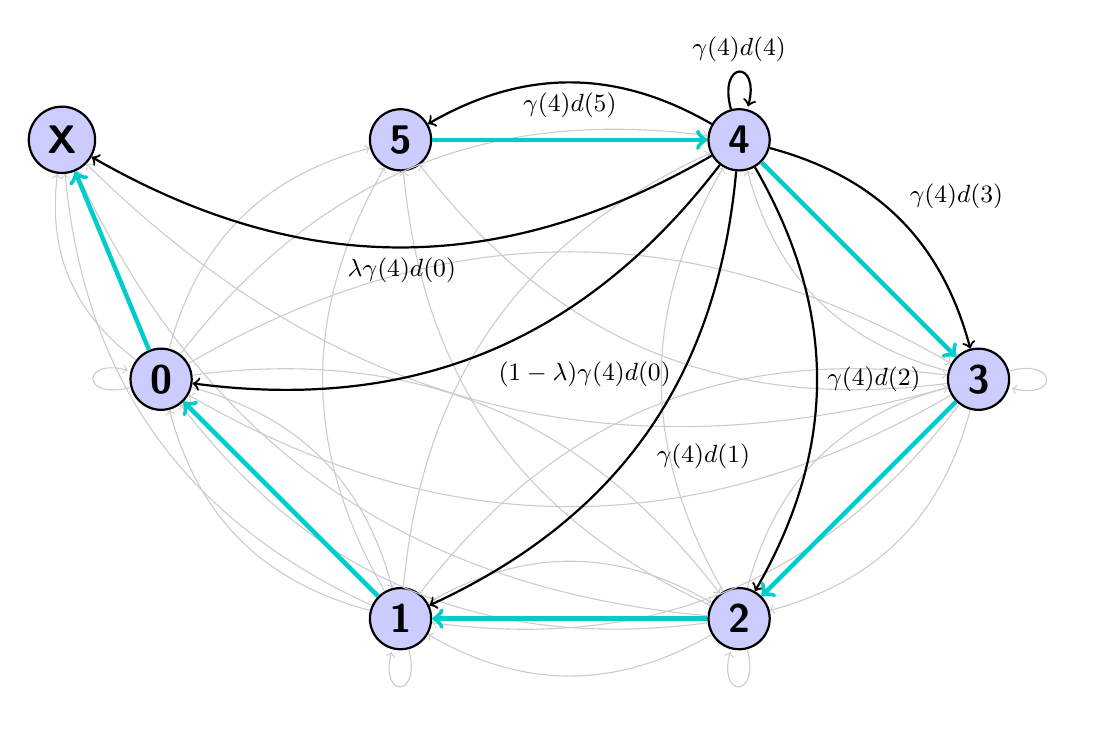
\begin{tikzpicture}[->,auto,node distance=4.3cm,thick,main
node/.style={circle,fill=blue!20,draw,font=\sffamily\Large\bfseries}]
  \definecolor{gray}{rgb}{0.8,0.8,0.8}
  \definecolor{lightgreen}{rgb}{0,0.8,0.8}
  
  \node[main node] (0) {0};
  \node[main node] (5) [above right of=0] {5};
  \node[main node] (4) [right of=5] {4};
  \node[main node] (3) [below right of=4] {3};
  \node[main node] (2) [below left of=3] {2};
  \node[main node] (1) [left of=2] {1};
  \node[main node] (X) [left of = 5] {X};

  \path[every node/.style={font=\sffamily\small},draw=gray,thin]
    (3) edge [bend left] node {} (5)
        edge [bend left] node {} (4)
        edge [bend left] node {} (2)
        edge [bend left] node {} (1)
        edge [bend left] node {} (0)  
        edge [bend left] node {} (X)
        edge [loop right] node {} (3) 
    (2) edge [bend left] node {} (5)
        edge [bend left] node {} (4)
        edge [bend left] node {} (3)
        edge [bend left] node {} (1)
        edge [bend left] node {} (0)     
        edge [loop below] node {} (2) 
        edge [bend left] node {} (X)
    (1) edge [bend left] node {} (5)
        edge [bend left] node {} (4)
        edge [bend left] node {} (3)
        edge [bend left] node {} (2)
        edge [bend left] node {} (0)    
        edge [loop below] node {} (1) 
        edge [bend left] node {} (X)
    (0) edge [bend left] node {} (5)
        edge [bend left] node {} (4)
        edge [bend left] node {} (3)
        edge [bend left] node {} (2)
        edge [bend left] node {} (1)
        edge [loop left] node {} (0) 
        edge [bend left] node {} (X);
        
    \path[every node/.style={font=\sffamily\small}]
    (4) edge [bend right] node {$\gamma(4)d(5)$} (5)
        edge [bend left] node {$\gamma(4)d(3)$} (3)
        edge [bend left] node {$\gamma(4)d(2)$} (2)
        edge [bend left] node {$\gamma(4)d(1)$} (1)
        edge [bend left] node {$(1-\lambda)\gamma (4)d(0)$} (0)
        edge [loop above] node {$\gamma(4)d(4)$} (4)
        edge [bend left] node {$\lambda \gamma(4)d(0)$} (X);
    
    \path[every node/.style={font=\sffamily\small}, ultra thick, color=lightgreen ] 
    (5) edge node {} (4)
    (4) edge node {} (3)
    (3) edge node {} (2)
    (2) edge node {} (1)
    (1) edge node {} (0)
    (0) edge node {} (X);    
\end{tikzpicture}
\end{figure}

%Thanatological age-classes will ideally terminate at the highest value
% permitted by data. For the data used in this paper, there are 111 total age classes, which
%translate to 111 total remaining-years classes (0-110+). In practice
% $\textbf{Y}$ becomes a 111$\times$111 matrix, with most entries non-zero (nearly complete
%connectivity, such as in Figure~\ref{fig:graph}). Construction may appear
% tedious for this reason. However, note that the bulk of fertility entries can be derived as the outer (tensor) product $d_a \otimes f_y$, leaving only the first row and first column mortality discounting followed by the addition of the
%survival superdiagonal. In most statistical programming languages constructing
% $\textbf{Y}$ entails only a couple more lines of code than constructing a Leslie matrix.

Thanatological projection matrices may be manipulated using
standard matrix techniques applicable to the Leslie matrix. Where $\textbf{p}$
is a population vector classified by thanatological age, projection proceeds by
multiplying $\textbf{Y}$ from the left:
$\textbf{p}(t + 1) = \textbf{Y}\textbf{p}(t)$. 

For rate schedules typical of human populations, thanatological projection
matrices are filled with non-negative values, mostly greater than zero. Raising
the matrix to some not-very-large power, $k$, will make all entries greater than zero. This observation, or else by noting that the
lifecylce graph is strongly connected, lets us conclude that the matrix is
irreducible and primitive. By the Perron-Frobenius theorem, the matrix will
 always have a unique, dominant, positive real eigenvalue, the natural
log of which is the intrinsic growth rate, $r$, and strong ergodicity is
assured.
In other words, given a fixed matrix and enough time, the population will conform to some stable thanatological age distribution. Strong
ergodicity was taken for granted in jumping from equation~\eqref{eq:ergostep1}
to ~\eqref{eq:ergostep2}, but the presently described properties of the matrix
model should, albeit unrigorously, satisfy lingering uncertainty on that step.
The eigenvector corresponding to the dominant eigenvalue gives this stable
thanatological age structure. If the fertility rates placed in the matrix are
from the stable population, then the growth rate from the thanatological
projection matrix is equal to that of the standard Leslie
matrix.\footnote{Some care needs to be taken in order to demonstrate this
point, since common approximations and adjustments used in matrix
construction can throw things off. \texttt{R} code is available from the
author to demonstrate this point. See also Appendix~\ref{app:B} for the
corresponding proof from the continuous model.} 

%The square of the ratio of
%the \nth{1} to the \nth{2} eigenvalues is the damping ratio, an indicator of
% the \textit{springiness} of the stable population structure, $c^\star(y)$, if perturbed from the
%state of stability.\footnote{See \citet[p.86-87]{caswell2001matrix}.} A higher
%damping ratio means that the population structure oscillates back to its stable
%state faster, i.e., that oscillations decrease in size more rapidly.
%Thanatological damping ratios are usually higher than chronological damping
%ratios in the data used elsewhere in this paper.

\section*{Stable age structure}
The thanatological stable age structure, as given in equation~\eqref{eq:cy},
displays some regular patterns worthy of mention. In Figuree~\ref{fig:str} the
same underlying mortality pattern, based on US males and females from 2010 (HMD) is rescaled to different mortality levels and growth
rates. Figure~\ref{tab:chronostr} shows stable age structures by chronological
age, while Figure~\ref{tab:thanostr} shows stable age structure of the same
population by thanatological age. Rows indicate growth rates, descending from
positive to negative, while columns indicate the both-sex mean life expectancy,
$e(0)$, to which 2010 US mortality is scaled. The rows and columns of
Figures~\ref{tab:chronostr} and \ref{tab:thanostr} are organized in identical
fashion, each element referring to the same intrinsic growth rate and average
$e(0)$.

The Brouard-Carey equality is visible by noting that the middle rows from the
chronological and thanatological matrices are identical. In comparing any other
rows, however, it is as if the thanatological matrix were flipped: a growingy is population in the chronological perspective looks like a shrinking
population in the thanatological perspective, and vice versa. While the bottom row of
Figure~\ref{tab:chronostr} looks like the top row of Figure~\ref{tab:thanostr},
the profiles ar enot rigorously identical, and the symmetry is only noteworthy
as rule of thumb. In thinking of the birth flow and the death flow, the
approximate reflection of age structure over the $r$-axis does make sense: in a
shrinking population new birth cohorts are smaller than old birth cohorts, which
means that relatively fewer people are born, and relatively more are in older
ages, closer to dying. In this case, the base of the chronological pyramid is
relatively thin, while the base of the thanatological leaf is relatively thick.
The same holds in reverse for growing populations. 

While this heuristic applies to stable populations, but it does not necessarily
hold for real observed populations under changing mortality. Further, the observation is only
valid for the period perspective in stability. In the cohort perspective, i.e.,
within closed birth cohorts, the analogy to stationary populations is spot on--- That is, within birth cohorts
the Brouard-Carey equality is exactly true when applied to the lifespan
distribution.
  
\begin{figure}[]
\centering
\caption{Stable age structures by life expectancy, $e(0)$, and growth rate,
$r$.*} \label{fig:str}
\begin{subfigure}[b]{\textwidth}
\centering
\caption{Chronological age structure, $c(a)$.}
\label{tab:chronostr}
\begin{tabular}{rccccc}
$e(0)\rightarrow$ \\
$\downarrow r $  & 55  & 65 & 75 & 85 & 95 \\
0.02  &\Py{0.02}{55}  &\Py{0.02}{65} &\Py{0.02}{75}&\Py{0.02}{85}  &\Py{0.02}{95}\\
0.01  &\Py{0.01}{55}  &\Py{0.01}{65} &\Py{0.01}{75} &\Py{0.01}{85} &\Py{0.01}{95}\\
0     &\Py{0}{55}     &\Py{0}{65}    &\Py{0}{75}    &\Py{0}{85}    &\Py{0}{95}\\
-0.01 &\Py{-0.01}{55} &\Py{-0.01}{65}&\Py{-0.01}{75}&\Py{-0.01}{85}&\Py{-0.01}{95}\\
-0.02 &\Py{-0.02}{55} &\Py{-0.02}{65}&\Py{-0.02}{75}&\Py{-0.02}{85}&\Py{-0.02}{95}
\end{tabular}
\end{subfigure}
\\ \vspace{2em}
\begin{subfigure}[b]{\textwidth}
\centering
\caption{Thanatological age structure, $c^\star(y)$.}
\label{tab:thanostr}
\begin{tabular}{rccccc}
$e(0)\rightarrow$ \\
$\downarrow r $  & 55  & 65 & 75 & 85 & 95 \\
0.02  &\Lf{0.02}{55}  &\Lf{0.02}{65} &\Lf{0.02}{75}&\Lf{0.02}{85}  &\Lf{0.02}{95}\\
0.01  &\Lf{0.01}{55}  &\Lf{0.01}{65} &\Lf{0.01}{75} &\Lf{0.01}{85} &\Lf{0.01}{95}\\
0     &\Lf{0}{55}     &\Lf{0}{65}    &\Lf{0}{75}    &\Lf{0}{85}    &\Lf{0}{95}\\
-0.01 &\Lf{-0.01}{55} &\Lf{-0.01}{65}&\Lf{-0.01}{75}&\Lf{-0.01}{85}&\Lf{-0.01}{95}\\
-0.02 &\Lf{-0.02}{55} &\Lf{-0.02}{65}&\Lf{-0.02}{75}&\Lf{-0.02}{85}&\Lf{-0.02}{95}
\end{tabular}
\end{subfigure}
\vspace{2em}
*Underlying mortality pattern based on 2010 USA (HMD)
\end{figure}
\FloatBarrier

%\section*{Some preliminary empirical findings}
%The thanatological renewal equation and the discrete projection matrix can be
%put to work with data. In this case a few options are available for determining
%what kind of thanatological fertility rates to use. The two obvious choices are
%to derive rates from the stable population implied by the chronological renewal
%model, or to derive rates such as those from Figure~\ref{fig:FySpaghetti},
%based on a particular stock of population. 

%Of the 1834 population-years of data on hand, we optimize $r$ from both
%\eqref{eq:thanoren} and \eqref{eq:lotka}. In this sample, both versions of $r$
%are only plausibly equal in a single instance. Usually thanatological $r$ is
%greater than Lotka's $r$ (1373 cases). When Lotka's $r$ is positive (693
% cases), thanatological $r$ is greater just over of 50\% of the time (356), but when Lotka's $r$ is negative, thanatological $r$ is the greater of the two around 90\% of the time (1017
%cases). These two approximations of $r$ are of opposite sign 138 times. We
%provide a comparison of the $r$ distributions in Figure~\ref{fig:rDist}. Mean
%locations for each distribution are indicated with vertical dashed lines;
% thano.
%-0.0010; chrono. -0.0027. The distribution of thanatological $r$ is more
% compact than for chronological $r$, with the ratio of variances (thano./chrono.) of
%about 0.75. The two theoretical values of $r$ covary strongly, but
%thanatological $r$ is the less erratic of the two, and it usually paints a less
% dire picture when both are negative.

%\begin{figure}[h!]
%	\caption{Distribution of $r$, chronological (Lotka) and thanatological*.}
%	\begin{center}
%		\label{fig:rDist}
%		\includegraphics[scale=.7]{Figures/rDist.pdf}
%	\end{center}
%	\begin{tiny}
 %    * Data from HMD and HFD. Countries and years listed in
  %   Figure~\ref{fig:Fxcompare}.
	%\end{tiny}
%\end{figure}

%The differences described here are not due primarily to rounding errors in the
%data, but rather to the way in which $\gamma(y)$ has been calculated. 
%Specifically, in this case we have transformed fertility rates from empirical
% data with a particular chronological age structure. If the chronological age structure is far from its
%stable distribution, then it may be hard to imagine that $\gamma(y)$ will
%remain fixed over time. When holding chronological-age classified fertility
% rates fixed, the assumption is just the opposite.

%From the projection matrix, the ratio of the largest to the second largest
%eigenvalue, the damping ratio, is an indicator of the \textit{springiness} of
%the stable population structure, $c^\star(y)$ or $c(a)$, if perturbed from the
%state of stability.
%A higher damping ratio means that the population structure oscillates back to
%its stable state faster, i.e., that oscillations decrease in size more rapidly.
% The thanatological damping ratio was greater than the Leslie damping ratio for all 1834 population-years included in
%our empirical analysis. Leslie damping ratios ranged from 1.01258 to 1.0518,
%while thanatological damping ratios ranged from 1.0455 to 1.0868. Again, this
%was for the raw data, and I am not sure whether this consistent finding is a
%natural property of the model or an artifact of the unstable starting state of
%the data used to derive thanatological fertility rates. Intuitively, the
%thanatological smoothing process should be an order of magnitude stronger than
%the chronological smoothing process because each thanatological age class
%(node) -- except for the oldest-old -- is connected directly to each other
%thanatological age class in both directions. Again, I think contrived examples
%will be necessary to shed more light on this finding.

\section*{Discussion}
The thanatological renewal model is valid, but I do not expect the reader to
accept that it is also a sound description of the fundamental forces of
population renewal. Specifically, I expect that the fertility rates are best
described in the margin by chronological age and not by thanatological age. The
main contribution of this inquiry is to demonstrate a transformation of the
Lotka-Leslie renewal model, and to highlight a parallel aspect of renewal that
occurs irrespective of its empirical regularity. That is, it is the case
that in the moment of birth, both progenitor and baby have a certain number of
remaining years of life, and that the range of potential values for both is
great. The thanatological renewal
model therefore is an abstraction of a real process, and not merely an adornment of the chronological renewal model.

What should one imagine under the model of thanatological population renewal? A useful mnemonic bases itself on Figures~\ref{fig:USdecomp} and \ref{fig:USrecomp}. In the chronological age-structured model, new generations appear at the bottom of the pyramid, and move up one class per year.
All age-classes are subject to attrition, which is spread out over ages and not
readily visible in the pyramid. In the thanatological \textit{leaf}, each birth cohort increments to the population over the whole range of thanatological age
according to $d(a)$, as seen in \eqref{eq:thanoren}, becoming the
shaded layers seen in Figure~\ref{fig:USrecomp}. Each horizontal step is a death
cohort, and these move one step down the pyramid each year without any decrement
(indeed incrementing due to births) until reaching the very bottom. In short,
the locations of increment and decrement, and the direction of movement (when
so visualized) are all swapped. The chronological and thanatological renewal
models are almost perfectly opposite descriptions of the same process. 

This symmetry is visible in comparing the
chronological and thanatological renewal equations~\eqref{eq:lotka2}
and \eqref{eq:thanoren}, and it is also seen in the approximate symmetry between
chronological and thanatological age structure profiles under intrinsic growth
rates of equal magnitude but opposite sign. The thanatological projection matrix may be thought of as a
sort of dual to the Leslie matrix--- a twin construct. The thanatological perspective on renewal I present is a hitherto undescribed property of the Lotka-Leslie renewal model. Possible applications of
this perspective on renewal are mentioned in \citet{riffe2015force}, the only
difference in the present inquiry is that we now account for constant growth rates in the
population. The present treatment is broader, and potentially applicable to a
wider range of birth-death processes. In the first place, we offer a deeper understanding
of the Lotka-Leslie renewal models.

\vspace{2em}

\begin{appendices}
\section{Unique solution for thanatological $r$}
\label{app:A}
This appendix contains a brief proof that the real solution for the
intrinsic growth rate, $r$, is unique for the case of the thanatological renewal model, \eqref{eq:thanoren}, and can be proven so in
essentially the same fashion as those in existence for the Lotka-Euler model,
\eqref{eq:lotka}. This proof follows that given in
\citet{pressat1973analyse}. Define a convenience function, $I(r)$, for the
integrand of \eqref{eq:thanoren} for a given $r$ and fixed $\gamma(y)$ and $d(a)$:

\begin{equation}
I(r) = \int_{y=0}^\infty \int_{a=0}^\infty \gamma(y) d(a+y)e^{-ra}\dd a \dd y
\end{equation}
Since the death distribution function, $d(a)$, and fertility
function, $\gamma(y)$, are continuous and non-negative, $\lim_{r \to +\infty} I(r)
= 0$ and $\lim_{r \to -\infty} I(r)= \infty$. If $r_2 > r_1$, then $I(r_1) >
I(r_2)$. $I()$ is therefore a continuous and monotonically decreasing function
of $r$ with boundaries that include the value 1 of \eqref{eq:thanoren}, and
 necessarily only obtain this value once. As with the Lotka-Euler equation, there will be more complex
 conjugate solutions for $r$ in the thanatological model,
 and these are not explored in this paper.


\section{Equivalence in stability}
\label{app:B}
This appendix contains a proof that the thanatological renewal equation implies
the same intrinsic growth rate, $r$, as the Lotka-Euler model if
the starting population is stable, given a particular set of thanatological
fertility rates.
This is identical to claiming that the right side of the renewal equation is
equal given the same $r$. Since there is a unique real solution, demonstrated in the previous appendix, then it is sufficient to
show that the two integral equations are equal under these conditions. The basic
relationship is:
\begin{align}
\int _{a=0}^\infty \ell(a)e^{-ra}f(a) \dd a &= \int _{y=0}^\infty \int
_{a=0}^\infty d(a+y)e^{-ra}\gamma (y) \dd a \dd y
\intertext{when}
\gamma(y) &= \frac{b^\star(y)}{c^\star(y)} \\
b^\star (y) &= \int_{a=0}^\infty b(a) \mu(a+y)\frac{\ell(a+y)}{\ell(a)} \dd a \\
c^\star (y) &= \int_{a=0}^\infty c(a) \mu(a+y)\frac{\ell(a+y)}{\ell(a)} \dd a
\intertext{Note that:}
c(a) &= \frac{\ell(a)e^{-ra}}{\int \ell(a) e^{-ra} \dd a} \\
b(a) &= m(a)c(a)
\end{align}Replacing $\gamma(y)$ with the full expanded
expression and plugging into the thanatological renewal equation gives:
\begin{align}
=& \int _{y=0}^\infty \int
_{a=0}^\infty d(a+y)e^{-ra} \frac{\frac{\int_{t=0}^\infty
m(t)\ell(t)e^{-rt}\mu(a+y)\frac{\ell(t+y)}{\ell(t)} \dd t}{\int \ell(t) e^{-rt} \dd
t}}{\frac{\int_{t=0}^\infty \ell(t)e^{-rt} \mu(t+y)\frac{\ell(t+y)}{\ell(t)} \dd t}{\int
\ell(t) e^{-rt} \dd t}} \dd a \dd y
\intertext{The denominator of $c(a)$ cancels out:}
=& \int _{y=0}^\infty \int
_{a=0}^\infty d(a+y)e^{-ra} \frac{
\int_{t=0}^\infty
m(t)\ell(t)e^{-rt}\mu(t+y)\frac{\ell(t+y)}{\ell(t)} \dd t}{
\int_{t=0}^\infty \ell(t)e^{-rt} \mu(t+y)\frac{\ell(t+y)}{\ell(t)} \dd t} \dd a \dd y
\intertext{Some $\ell(a)$'s also cancel out:}
=& \int _{y=0}^\infty \int
_{a=0}^\infty d(a+y)e^{-ra} \frac{
\int_{t=0}^\infty
m(t)e^{-rt}\mu(t+y)\ell(t+y) \dd t}{
\int_{t=0}^\infty e^{-rt} \mu(t+y)\ell(t+y) \dd t} \dd a \dd y
\intertext{Now $d(a+y) = \mu (a+y)\ell(a+y)$, so we can cancel the inner integral
with the denominator:}
=& \int _{y=0}^\infty 
\int_{a=0}^\infty
m(a)e^{-ra}\mu(a+y)\ell(a+y) \dd a \dd y
\intertext{Note also that $l(a) = \int _{=a}^\infty d(x) \dd x$ (present
livings are future deaths), which brings us back to the chronological
formulation:} =& \int_{a=0}^\infty e^{-ra}\ell(a)m(a)
\dd a
\end{align}
This proof establishes that in the stable population there is at least
one thanatological fertility rate schedule that will satisfy the constraints of
the lifespan distribution and $r$. However, it is not necessary to derive the
thanatological fertility distribution in the way prescribed here, and indeed an
infinite number of such fertility distributions would satisfy the same
constraints. Imagine these fertility rates cross-classified in
both age dimensions, where two marginal sums give the thanatological and
chronological rates, as they would be calculated over the
corresponding cross-classified exposures. The shape of this rate surface can be
shifted around in infinitely many ways that would preserve a given growth rate
and lifespan distribution, and the above proof shows one such mapping.

\section{An iterative method to find the thanatological $r$}
\label{app:C}
\citet{coale1957new} proposed a fast-converging iterative approach to estimate
the intrinsic growth rate for the Lotka-Euler equation. For the thanatological
renewal model, a similar approach may be taken, with some slight
modifications to Coale's original.
The following steps can be followed to estimate $r$ from
Equation~\eqref{eq:thanoren}:

\begin{enumerate}
  \item Derive a first rough estimate of the mean remaining years of life at
  reproduction, $\widehat{T^\star}$, akin to Lotka's mean generation time, $T$.
  To start, a good-enough guess is to just assume $r=0$:\footnote{Using the
  Brouard-Carey equality, the denominator could also be: $\int _{y=0}^\infty
  \ell(y) \gamma(y) \dd y$}
\begin{equation}
\widehat{T^\star} = \frac{\int _{y=0}^\infty \int _{a=0}^\infty y d (a+y)
\gamma(y) \dd a \dd y}{\int _{y=0}^\infty \int _{a=0}^\infty d(a+y) \gamma(y)
\dd a \dd y}
\end{equation}
  \item A first rough guess at the net reproduction rate, $R_0^\star$ is given
  by
 \begin{equation}
  R_0^\star = \int _{y=0}^\infty \int _{a=0}^\infty d(a+y) \gamma(y) \dd a
\dd y
\end{equation}
  \item A first rough estimate of $r$, $r^0$, is given by
   \begin{equation}
   r^0 = \frac{ln(R_0^\star)}{\widehat{T^\star}}
   \end{equation}
  \item Plug $r^0$ into Equation~\eqref{eq:thanoren} to calculate a
  residual, $\delta^0$.
  \item Use $\delta^0$ and $\widehat{T^\star}$ to calibrate the estimate of $r$
  using
  \begin{equation}
  r^{1} = r^0 + \frac{\delta^0}{\widehat{T^\star} - \frac{\delta^0}{r^0}}
  \end{equation}
  \item Repeat step (4) to to derive a new $\delta^i$, then step (5) to refine
  $r^i$, until converging on a stable $r$ after some 20 or so iterations,
  depending on the degree of precision desired ($\widehat{T^\star}$ is not updated
  in this process).
\end{enumerate}

The above procedure is more computationally efficient than minimizing the
absolute residual of Equation~\eqref{eq:thanoren} using a generic
optimizer. Alternatively, one could use the method of cumulants to estimate $r$,
but this would entail less precision than the above (unless one goes beyond,
say, five cumulants), and this is not explored.
 
 
\end{appendices}
\nocite{HMD,HFD}
-------------------------
% bibliography
\bibliographystyle{plainnat}
  \bibliography{References}  

\end{document}
